\documentclass[12pt, oneside]{article}
\usepackage[letterpaper]{geometry}
\usepackage{Logemann}
\usepackage{SetTheory}
\usepackage{Sum}
\usepackage{Product}
\usepackage{listings}
\usepackage{jlcode}

\begin{document}
\noindent \textbf{\Large{Caleb Logemann \\
AERE 504 Intelligent Air Systems \\
Project 1
}}

\section{Description of Methods}
  For this project I implemented both the k2 search algorithm and the local
  search algorithm.
  The k2 algorithm starts with a ordering of the variables and then generates
  a Bayesian Network structure that maximizes the Bayesian score and such that
  the ordering is a topological sort of the nodes.
  The local search algorithm starts from a random structure and then takes
  local moves to maximize the Bayesian score.

  For my full search algorithm I used a combination of both of these algorithms.
  I first generated a random ordering of variables and then applied the k2 algorithm.
  I then used the local search on the result of the k2 search.
  This can only improve upon the result of the k2 algorithm and guarantees that
  I am at a local maximum.
  I also used a randomized restarting process to more fully search the space
  and to make sure the algorithm didn't get stuck at a poor local maximum.
\section{Graphs and Scores}
  \begin{center}
    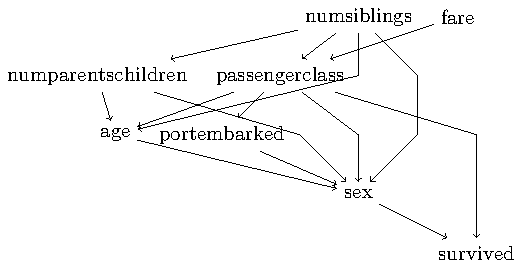
\includegraphics[scale=0.8]{titanic.pdf}
  \end{center}
  The Bayesian Score for this structure is .
  It took XXXXX seconds to compute a 1000 random restarts.
  \begin{center}
    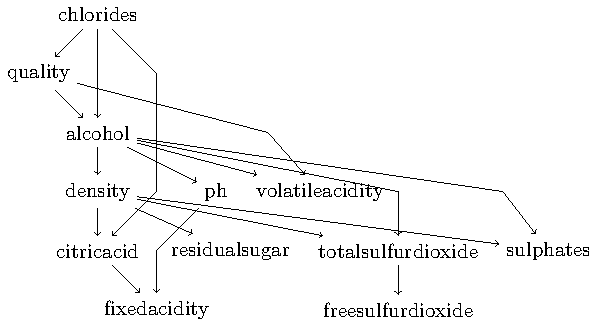
\includegraphics[scale=0.8]{whitewine.pdf}
  \end{center}
  The Bayesian Score for this structure is .
  It took XXXXX seconds to compute a 500 random restarts.
  \begin{center}
    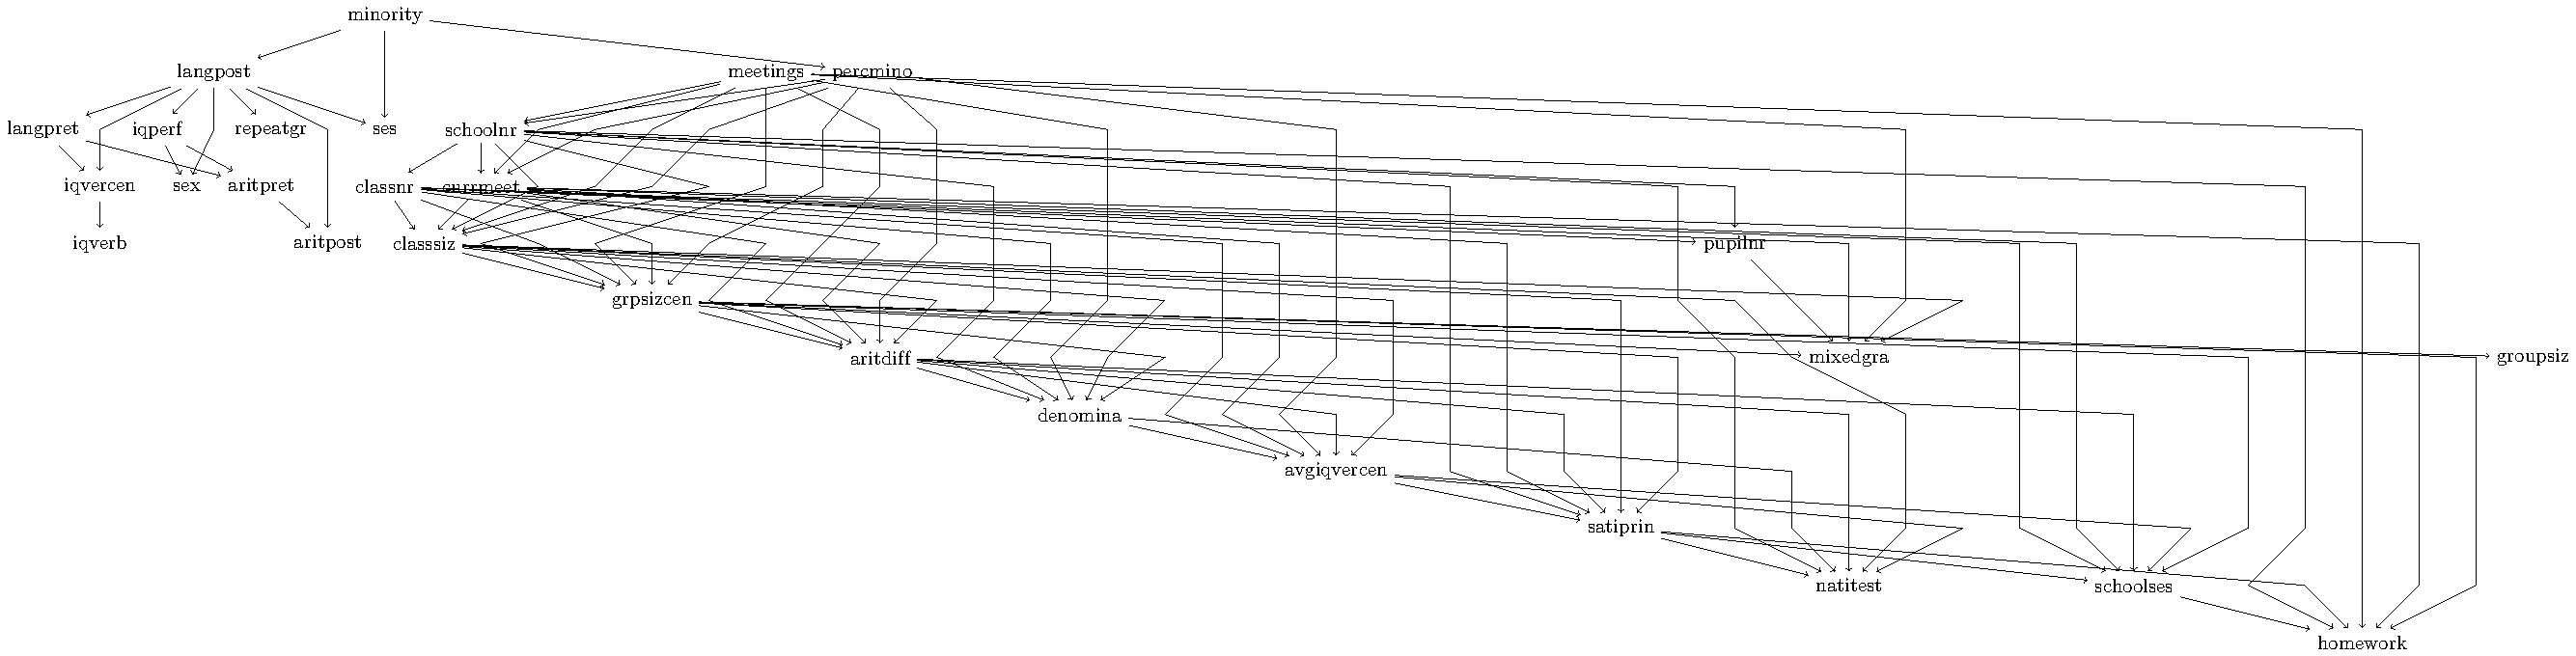
\includegraphics[scale=0.4]{schoolgrades.pdf}
  \end{center}
  The Bayesian Score for this structure is .
  It took XXXXX seconds to compute a 100 random restarts.
  %\begin{center}
    %\includegraphics[scale=0.5]{structuredlearning_test.pdf}
  %\end{center}
  The Bayesian Score for this structure is .
  It took XXXXX seconds to compute a 1000 random restarts.

  \lstinputlisting[breaklines=true]{Project1.jl}
  \lstinputlisting[breaklines=true]{BayesianNetworks.jl}

\end{document}

